\documentclass[11pt]{report}
\usepackage{geometry}        
\geometry{a4paper}    
\usepackage[parfill]{parskip}  
\usepackage{graphicx}
\usepackage{amsmath, amssymb, amsthm}
\usepackage{siunitx}
\usepackage{tikz, pgfplots}
\usepackage{epstopdf}
\DeclareGraphicsRule{.tif}{png}{.png}{`convert #1 `dirname #1`/`basename #1 .tif`.png}

\usepackage[colorlinks=true, pdfstartview=FitV, linkcolor=blue, 
            citecolor=blue, urlcolor=blue]{hyperref}

%\includeonly{Chapter1}


\theoremstyle{definition}
\newtheorem{theorem}{Theorem}
\newtheorem{corollary}[theorem]{Corollary}
\newtheorem{definition}{Definition}
\newtheorem{lemma}{Lemma}
\newtheorem{exercise}{Exercise}
\newtheorem{remark}{Remark}
\newtheorem{example}{Example}
\newtheorem{warning}{Warning}

\newcommand{\harpoon}{\overset{\rightharpoonup}}

\def\grad{ \mbox{grad}}
\def\curl{ \mbox{curl}}
\def\div{ \mbox{div}}
\def\U{\ensuremath {\cal U}}
\def\S{\ensuremath {\cal S}}
\def\V{\ensuremath {\cal V}}
\def\R{\ensuremath {\cal R}}
\def\tr{\ensuremath {\mbox{tr}}}

\pagenumbering{arabic}



% ------------------- Title and Author -----------------------------
\title{Physics Notes}
\author{Author}
\begin{document}


\maketitle

\tableofcontents

\chapter[Practical Skills]{Development of Practical Skills in Physics}
\include{chapter-1}

\chapter[Foundations of Physics]{Foundations of Physics}
\include{chapter-2}

\chapter[Forces and Motion]{Forces and Motion}
% Activate the following line by filling in the right side. If for example the name of the root file is Main.tex, write
% "...root = Main.tex" if the chapter file is in the same directory, and "...root = ../Main.tex" if the chapter is in a subdirectory.
 
%!TEX root = phys-notes.tex

\section{Motion}

\subsection{Definitions}

Kinematics is the study of motion. It refers only the motion of objects and the positions, without considering their masses or forces.

\begin{definition}
	Displacement is the distance moved in a particular direction from a reference point. It is a vector quantity.
\end{definition}

\begin{definition}
	Velocity is displacement per unit time. It is the first derivative of displacement with respect to time ($\frac{ds}{dt}$), and is a vector quantity.
\end{definition}

\begin{definition}
	Acceleration is change in velocity per unit time. It is the second derivative of displacement w.r.t. time ($\frac{d^2s}{dt^2}$), and is a vector quantity.
\label{def:accel}
\end{definition}

\subsection{Graphs of motion}

Imagine throwing an object vertically into the air. These are its displacement, velocity, and acceleration graphs:

\begin{figure}[ht]
\begin{tabular}{c c c}
	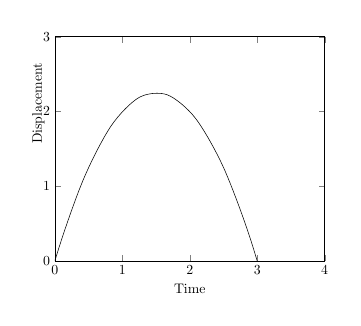
\begin{tikzpicture}[scale=0.5]
		\begin{axis}[xmin=0, ymin=0, xmax=4, ymax=3,
					 xlabel={Time}, xlabel style={below},
					 ylabel={Displacement}, ylabel style={right}]
			
			\addplot[mark=none, smooth] {-x^2+3*x};
		\end{axis}
	\end{tikzpicture}
	&
	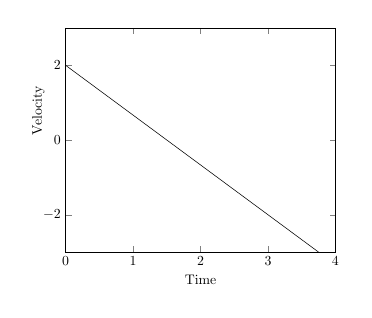
\begin{tikzpicture}[scale=0.5]
		\begin{axis}[xmin=0, ymin=-3, xmax=4, ymax=3,
					 xlabel={Time}, xlabel style={below},
					 ylabel={Velocity}, ylabel style={right}]
			
			\addplot[mark=none, smooth] {-(4/3)*x + 2};
		\end{axis}
	\end{tikzpicture}
	&
	\begin{tikzpicture}[scale=0.5]
		\begin{axis}[xmin=0, ymin=-3, xmax=4, ymax=3,
					 xlabel={Time}, xlabel style={below},
					 ylabel={Acceleration}, ylabel style={right}]
			
			\addplot[mark=none, smooth] {-2};
		\end{axis}
	\end{tikzpicture}
\end{tabular}
\caption{Graphs for a ball being thrown}
\end{figure}

We can see from this that when the displacement graph is a curve, the velocity is changing at a constant rate. If the velocity is a curve, acceleration is changing at a constant rate. The gradient of a displacement-time graph gives velocity, and the gradient of a velocity time graph gives acceleration. 

The reverse is also true: the area under the curve of an acceleration-time graph gives velocity, and the area under a velocity-time graph gives displacement. In calculus terms, the integral of acceleration with respect to time is velocity.

\subsection{Constant Acceleration Equations}

Motion with invariant acceleration can be described using a family of equations. Each of these use a combination of five variables:

\begin{itemize}
	\item $s$: displacement.
	\item $u$: initial velocity.
	\item $v$: final velocity.
	\item $a$: acceleration.
	\item $t$: time.
\end{itemize}

Each suvat equation uses four of these, meaning that all parameters can be calculated if we know only three.

\begin{definition}
	Suvat equations: $v=u+at$, $s=ut+\frac{1}{2}at^{2}$, $s=vt-\frac{1}{2}at^{2}$, $v^{2}=u^{2}+2as$, and $s=\frac{1}{2}(u+v)t$.
\end{definition}
We can combine, rearrange and evaluate these for different systems. It's important to note that sign is important. If you say that $a=-9.81$ then downward displacement should be negative.

\subsection{Projectile Motion}

Imagine a ball thrown horizontally from a height (maybe a cliff or a tower). It has some initial velocity $u$ and an initial height. The following is a diagram of the scenario.

\begin{figure}[ht]
\centering
	\begin{tikzpicture}
		\begin{axis}[xmin=-0.3, ymin=0, xmax=3, ymax=5, 
					 xticklabels={}, yticklabels={},
					 axis line style={draw=none}, tick style={draw=none},
					 smooth]
			
			%Trajectory
			\addplot[mark=none, red, very thick, domain=0:4] {-0.7*x^2+4};
			\addplot[mark=none, black, thick, domain=0:4] {0};
			
			%Nodes
			\node[circle, fill=black, minimum size=2mm, inner sep=0pt] (start) at (axis cs: 0,4){};
			\node (v) at (axis cs: 1.2,4){};
			\node (h) at (axis cs: 0,0){};
			\node[label=above:$v$] (v_label) at (axis cs: 0.6,4) {};
			\node[label=left:$s_{y}$] (h_label) at (axis cs: 0,2) {};
			
			%Draw
			\draw[-stealth, thick] (start) -- (v);
			\draw[|-|, thick] (start) -- (h.center);
		\end{axis}
	\end{tikzpicture}
	\caption{A ball is thrown with a horizontal velocity $v$ from a height $s_{y}$.}
\end{figure}

The time that the ball is in the air is, counter-intuitively, solely dependent on $s_{y}$ and on $a$, the acceleration. The time that it will take the ball to hit the ground is calculated as follows:
\[s_{y}=ut+\frac{1}{2}at^{2} \Rightarrow t=\sqrt{\frac{2s_{y}}{a}}\]
And the horizontal distance to the point of impact with the ground is given by:
\[v=\frac{s}{t} \Rightarrow s=vt\]

Now, consider a different scenario. The ball is now projected from the ground, with an initial velocity $v$ at an angle $\theta$ from the horizontal.

\begin{figure}[ht]
\centering
	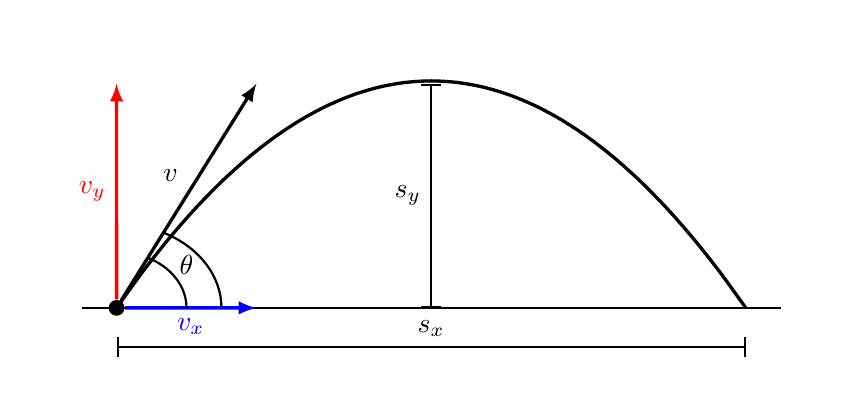
\begin{tikzpicture}
		\begin{axis}[xmin=-1, ymin=-1, xmax=10, ymax=5, yscale=0.5*1.5, xscale=0.95*1.5,
					 xticklabels={}, yticklabels={},
					 axis line style={draw=none}, tick style={draw=none},
					 smooth]
			
			%Trajectory
			\addplot[mark=none, black, very thick, domain=0:9] {-0.2*x^2+1.8*x};
			\addplot[mark=none, black, thick, domain=-0.5:9.5] {0};
			
			%Nodes
			\node[circle, fill=black, minimum size=2mm, inner sep=0pt] (start) at (axis cs: 0,0){};
			\node (max) at (axis cs: 4.5,4.05) {};
			\node[label=$\theta$] (angle_label) at (axis cs: 1,0.24) {};
			
			%Draw
			\draw[-latex, very thick] (start) -- (axis cs: 2,4) node [midway, above left] {$v$};
			\draw[-latex, very thick, blue] (start) -- (axis cs: 2,0) node [midway, below] {$v_{x}$};
			\draw[-latex, very thick, red] (start) -- (axis cs: 0,4) node [midway, left] {$v_{y}$};
			\draw[thick] (axis cs:1,0) arc (0:63:1);
			\draw[|-|, thick] (axis cs: 4.5,0) -- (axis cs: 4.5,4) node [midway, left] {$s_{y}$};
			\draw[|-|, thick] (axis cs: 0,-0.7) -- (axis cs: 9,-0.7) node [midway, above] {$s_{x}$};
			\draw[thick] (axis cs: 1.5,0) arc (0:63:1.5);
		\end{axis}
	\end{tikzpicture}
	\caption{A ball is thrown with a horizontal velocity $v$ at an angle $\theta$.}
\end{figure}

A fundamental principle is that the perpendicular components of velocity are independent of each other. The horizontal velocity $v_{x}$ is constant, and the vertical velocity $v_{y}$ is dependent on acceleration. This means that, again, time is solely dependent on $v_{y}$, and the horizontal distance on $v_{x}$. First, we need to resolve the velocity. Using trigonometry:
\[v_{x}=v\cos\theta\]
\[v_{y}=v\sin\theta\]
At the maximum of the curve, or the highest point, $v_{y}=0$. This makes sense, since it is the moment where the ball changes direction (and is when $\frac{ds}{dt}=0$). Knowing this fact, we can use $v^{2}=u^{2}+2as$ to calculate $s_{y}$:
\[v^{2}=u^{2}+2as \Rightarrow s_{y}=\frac{0-u^{2}}{2a}\]
Now that we know the maximum height, notice that the second half of this trajectory is identical to the scenario with horizontal motion. We can now use the same logic to find the time for the ball to drop from this point to the ground (i.e. the time for the second half of the trajectory)
\[s_{y}=ut+\frac{1}{2}at^{2} \Rightarrow t=\sqrt{\frac{2s_{y}}{a}}\]
Notice that when the start and end height are the same, the trajectory is symmeterical. This means that the time for the ball to reach the maximum point is the same as how long it takes for it to fall. Therefore, its total flight time is $2t$. Knowing this, we can calculate $s_{x}$. Horizontal velocity is constant so:
\[s_{x}=2tv_{x}\]

\section{Forces}

\subsection{The Newton}

\begin{definition}
	The newton ($\si{\newton}$, base units $\si{\kilo\gram\meter\per\second\squared}$) is the unit of force. One newton is the force required to give a mass of one kilogram an acceleration of one meter per second.
\end{definition}

The most fundamental equation of forces is derived from Newton's Second law of motion. It describes the simple relationship between the force an object feels, its mass and its acceleration.
\begin{equation}
	\sum\vec{F} = m \vec{a}
	\label{eq:newton}
\end{equation}
The force in this equation is the sum of the forces, or the net/resultant force on the object. This is shown in Figure \ref{fig:example}. In this case, the acceleration is felt in the direction of the net force. However, this does not mean that it is moving in this direction; the acceleration could be slowing it down, or changing it's direction of motion, we do not have the information necessary to determine what is the case.  

\begin{figure}[ht]
	\centering
	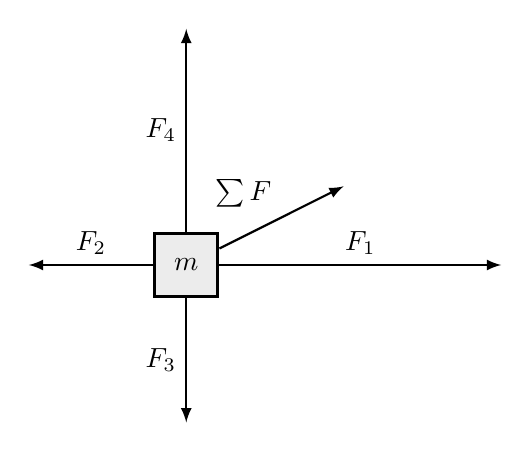
\begin{tikzpicture}
		%Node
		\node[rectangle, fill=gray!15, draw, minimum size=8mm, very thick] (obj) at (0,0) {$m$};
		
		%Vectors
		\draw[-latex, thick] (obj) -- (4, 0) node [midway, above] {$F_{1}$};
		\draw[-latex, thick] (obj) -- (-2,0) node [midway, above] {$F_{2}$};
		\draw[-latex, thick] (obj) -- (0,-2) node [midway, left] {$F_{3}$};
		\draw[-latex, thick] (obj) -- (0, 3) node [midway, left] {$F_{4}$};
		\draw[-latex, thick] (obj) -- (2, 1) node [midway, above left] {$\sum F$};
	\end{tikzpicture}
	\caption{Example free-body diagram}
	\label{fig:example}
\end{figure}

Newton's original second law defined the force as the rate of change in momentum with respect to time. We can simplify the differential to find Eq. \label{eq:newton}.
\[\vec{p}=m\vec{v} \text{ so } \sum\vec{F}=\frac{dm\vec{v}}{dt}\]
Factor out $m$:
\[\sum\vec{F}=m\frac{d\vec{v}}{dt} = m\vec{a}\]
by Definition \ref{def:accel}.

\subsection{Center of Mass}

The center of mass of an object is the point at which its mass appears to be concentrated. A force applied to this point causes the object to accelerate linearly. This means we also draw forces coming out of this point. The height of the center of mass is one of the two factors that determine the stability of an object. The other is the size of the base area. If the line of force passses through the base of the object, it will not topple. If it passes outside of this area it will fall over (Fig. \ref{fig:boxes}). Arc length is found by multiplying its corresponding angle by the radius. It so follows that the higher the center of mass is, the more unstable it is, since a smaller angle is capable of pushing the line of force outside of the base area.

\begin{figure}[ht]
\centering
	\begin{tabular}{c c}
		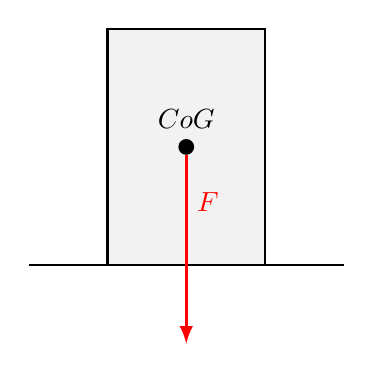
\begin{tikzpicture}
			\draw[thick] (-2,0)--(2,0);
			\draw[thick, fill=gray!10] (-1,0)--(1,0)--(1,3)--(-1,3)--(-1,0);
			\node[circle, fill=black, minimum size=2mm, inner sep=0pt, label=$CoG$] (cog) at (0,1.5){};
			\draw[-latex, very thick, red] (cog)--(0,-1) node [near start, right] {$F$};
		\end{tikzpicture}
		&
		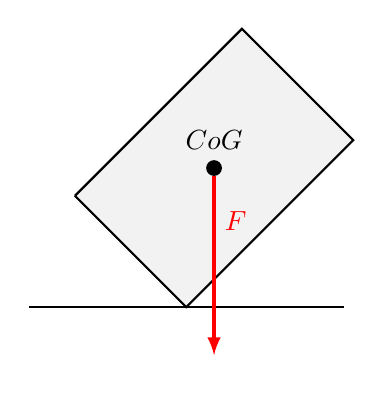
\begin{tikzpicture}
			\draw[thick] (-1,0)--(3,0);
			\begin{scope}[shift={({1-cos(45)},{sin(45)})}]
				\draw[thick, fill=gray!10, rotate=-45] (-1,0)--(1,0)--(1,3)--(-1,3)--(-1,0);
			\end{scope}
			\node[circle, fill=black, minimum size=2mm, inner sep=0pt, label=$CoG$] (cog) at (1+0.353,1.767){};
			\node[] (f) at (1+0.353,1.767-2.5){};
			\draw[-latex, very thick, red] (cog)--(f) node [near start, right] {$F$};
		\end{tikzpicture}
	\end{tabular}
	\caption{Boxes. The first is stable, the second is not.}
	\label{fig:boxes}
\end{figure}



\chapter[Electrons, Waves, and Photons]{Electrons, Waves, and Photons}
% Activate the following line by filling in the right side. If for example the name of the root file is Main.tex, write
% "...root = Main.tex" if the chapter file is in the same directory, and "...root = ../Main.tex" if the chapter is in a subdirectory.
 
%!TEX root = phys-notes.tex

\section{Charge and Current}

\subsection{Charge}

Charge is a fundamental property of certain particles. Some particles (protons) have positive charge, some (electrons) have negative charge. Charge is quantized, so the charge of any particle or atom is an integer multiple of the elementary charge (Def. \ref{def:e}).

An electric current consists of a flow of charged particles. Electric current is the rate of flow of charge:
\begin{equation}
	I=\frac{\Delta Q}{\Delta t}
	\label{eq:chargedef}
\end{equation}
Charge $Q$ is measured in coulombs, and time $t$ is measured in seconds. Current $I$ is measured in amperes.

\begin{definition}
	Kirchhoff's First Law: Since charge is always conserved, the sum of the charges flowing into a circuit junction is equal to the sum of the charges leaving it. Stated mathematically: $\sum{I_{in}} = \sum{I_{out}}$. Or, as vector quantities, $\sum{I_{in}} + \sum{I_{out}} = 0$.
\end{definition}

\begin{definition}
	The elementary charge $e$ is the charge of a single electron and has a value of $1.6\times10^{-19}\si{\coulomb}$.
	\label{def:e}
\end{definition}

Since the coulomb is defined as the quantity of charge that passes a fixed point in one second, we can find the amount of electrons in a single coulomb ($\frac{1}{e}$), or by extension the amount of electrons passing a point in a fixed amount of time. 

\subsection{Electron Drift Velocity}

Metals, at an atomic level, are structured as a crystalline lattice. Atoms are bonded together and spaced out at regular intervals. Around them are delocalised electrons that are free to move in the lattice. These are also called conduction electrons. The more conducting electrons a metal has, the more conducive it is. Electrons always move randomly.

When no potential difference is applied to a metal, there is no current. This means electrons move randomly with no net motion. When a potential difference is applied to a metal, a current flows. Electrons move randomly and slowly; however, there is a net motion from - to +. This net motion is the drift velocity being superimposed on the random velocities of the electrons.

\begin{definition}
	Calculation of electron drift velocity. Current can be calculated as charge over time. By considering the dimensions of the wire we can arrive at an equation for current:
\begin{equation}
	I=nAev
	\label{eq:driftv}
\end{equation}
\end{definition}
$I$ is the current, $n$ is the number density of electrons, $A$ is the cross-subsectional area of the wire, $e$ is the elementary charge, and $v$ is the drift velocity of electrons. The charge available is the amount of electrons ($nAL$, where $L$ is the length of the wire) multiplied by the charge of each electron $e$. The time for the charge to travel the length $L$ is $\frac{L}{v}$. So, by using the charge equation for current (Eq. \ref{eq:chargedef}), we arrive at $I=nAev$. This equation also illustrates other properties. It is apparent from it that $v \propto\frac{1}{n}$. We can physically understand this in terms of electrons; the less particles there are in a given space, the further an electron can move and accelerate without colliding into another particle.

Metals have a high number density of electrons (around $\times 10^{28}$), and so are good conductors. Semi conductors have less (around $\times 10^{10}$), and so are less conductive. Insulators have close to zero conducting electrons, so do not conduct.

\section{Energy, Power, and Resistance}

\subsection{Potential Difference and Electromotive Force}

\subsubsection{Definitions of P.D and E.M.F}
In order for electric current to flow in a circuit, there must be a source of energy.

\begin{definition}
	Electromotive Force (e.m.f) is the potential difference across the power supply. It is a measure of the external energy (usually chemical) that is being transferred to the electrical energy of the circuit.
\end{definition}

\begin{definition}
	The potential difference (p.d) across each component describes how much energy per unit charge is being transferred at each component.
\end{definition}

We can think of e.m.f as describing input energy, and p.d as describing output energy. Both can be measured in joules per coulomb ($\si{\joule\per\coulomb}$) or in $\si{\volt}$. E.m.f is energy transferred per unit charge, while p.d. is work done per unit charge.\\
Equation for e.m.f:
\begin{equation}
	\varepsilon = \frac{W}{Q}
	\label{eq:emfdef}
\end{equation}
where $W$ is energy transferred (in Joules) and $Q$ is charge (in Coulombs).\\

Equation for p.d:
\begin{equation}
	V = \frac{W}{Q}
	\label{eq:pddef}
\end{equation}
where $W$ is work done and $Q$ is charge.

\subsubsection{The Electron Gun and the Electron Volt}

An electron has charge $e$, so it undergoes an energy change of $eV$ as it passes a p.d $V$. When a potential difference is applied to a conductor, electrons are accelerated and gain kinetic energy. When this p.d. is $V$, the kinetic energy gained can be expressed as:
\begin{equation}
	eV=\frac{1}{2}m_{e}v^2
	\label{eq:eaccel}
\end{equation}
where $m_e$ is the mass of an electron.

\subsection{Resistance and Ohm's Law}

\subsubsection{Defining Resistance}
\begin{definition}
	Ohm's Law: The current through a conductor is directly proportional to the potential difference across it, provided that physical conditions remain constant.
\end{definition}

Resistance is defied as the opposition to current. It is described by:
\begin{equation}
	R = \frac{V}{I}
	\label{eq:ohmslaw}
\end{equation}
and has the units Ohm ($\si{\ohm}$). An ohmic conductor (wire, resistor) is one that follows Ohm's Law. It's I-V graph should be a straight line. To determine the resistance from an I-V graph, find the reciprocal of its gradient.

The resistance of a wire is directly proportional to the length and inversely proportional to the cross subsectional area.

\subsubsection{I-V Characteristic of Components}

The I-V characteristics of various components can be experimentally investigated using a circuit with a power supply, ammeter, variable resistor, and component in series. A voltmeter should also be wired around the component. The variable resistor can be used to vary current, and an I-V graph can be plotted.\\

Wire and conductor (Fig. \ref{fig:wireIV}): At a constant temperature, these follow Ohm's law. They behave the same way regardless of the direction of current, so their I-V graphs are a straight line.

\begin{figure}[ht]
	\centering
	\begin{tikzpicture}[scale=0.8]
		\begin{axis}[axis x line=center, axis y line=center, domain=-5:5, xticklabels={}, yticklabels={},
					 xlabel={Potential Difference $V$}, ylabel={Current $I$}, 
					 xlabel style={below}, ylabel style={above left},]
					 
    		\addplot [mark=none, domain=-3:3] {x};
    	\end{axis}
	\end{tikzpicture}
	\caption{I-V characteristic of a wire}
	\label{fig:wireIV}
\end{figure}

Filament Lamp (Fig. \ref{fig:bulbIV}): As the current increases, electron velocity is increase. This leads to a higher rate of more energetic collisions between electrons and the metal structure. The collisions cause the metal ions to have a higher vibrational kinetic energy (i.e. increasing temperature). This increases the probability of a collision, and increases the resistance. The process repeats and repeats. At low current, the bulb approximates Ohm's law. It does not obey Ohm's law at high currents, so its graph is non-linear.

\begin{figure}[ht]
	\centering
	\begin{tikzpicture}[scale=0.8]
		\begin{axis}[axis x line=center, axis y line=center, domain=-5:5, xticklabels={}, yticklabels={},
					 xlabel={Potential Difference $V$}, ylabel={Current $I$}, 
					 xlabel style={below}, ylabel style={above left},]
					 
    		\addplot [mark=none, domain=-3:3] {1/(1+e^(-1.3*x))-0.5}; 
    	\end{axis}
	\end{tikzpicture}
	\caption{I-V characteristic of a filament bulb}
	\label{fig:bulbIV}
\end{figure}

Diode or LED (Fig. \ref{fig:diodeIV}): These depend on the polarity of the battery, since they let current flow only one way. In the forward bias direction, they follow ohm's law, while in the reverse bias they have an almost infinite resistance. 

\begin{figure}[ht]
	\centering
	\begin{tikzpicture}[scale=0.8]
		\begin{axis}[axis x line=center, axis y line=center, domain=-5:5, xticklabels={}, yticklabels={},
					 xlabel={Potential Difference $V$}, ylabel={Current $I$}, 
					 xlabel style={below}, ylabel style={above left},]
					 
			\addplot [mark=none, domain=-3:0.3] {0}; 
    		\addplot [mark=none, domain=0.3:3] {x-0.3}; 
    	\end{axis}
	\end{tikzpicture}
	\caption{I-V characteristic of a diode}
	\label{fig:diodeIV}
\end{figure}

Thermistor and LDR (Fig. \ref{fig:ldrIV}): These respond to external conditions and have an inverse relationship:

\begin{figure}[ht]
	\centering
	\begin{tikzpicture}[scale=0.8]
		\begin{axis}[axis x line=center, axis y line=center, domain=0:5, xticklabels={}, yticklabels={},
					 xlabel={Temprature/Light Intensity}, ylabel={Resistance}, 
					 xlabel style={below}, ylabel style={above left},]
					 
    		\addplot [mark=none, domain=0:5] {1/x}; 
    	\end{axis}
	\end{tikzpicture}
	\caption{Characteristic of a thermistor/LDR}
	\label{fig:ldrIV}
\end{figure}

\subsection{Resistivity}

The resistance of a material depends on its physical conditions and dimensions.

\begin{definition}
	Resistivity is an intrinsic property of a material, irrespective of its physical shape. It is given in units Ohm meters ($\si{\ohm\meter}$) and calculated using the equation:
	\begin{equation}
		\rho = \frac{RA}{l}
		\label{eq:resistivity}
	\end{equation}
\end{definition}

\subsection{Power}

\subsubsection{Power Fundamentals}

\begin{definition}
	Power is the rate at which energy is transferred from one form to another. The unit of power is the watt, ($\si{\watt}$). $1\si{\watt}=\frac{1\si{\joule}}{1\si{s}}$.
\end{definition}

By combining the above definition of power with the definition of the Volt (Eq. \ref{eq:pddef}) and Ohm's law (Eq. \ref{eq:ohmslaw}), we arrive at the three equations for power:
\begin{eqnarray}
	P=IV\\
	\label{eq:poweriv}
	P=I^2R\\
	P=\frac{V^2}{R}
\end{eqnarray}
Recall a previous equation for power, $P=\frac{E}{t}$. With this, we can relate energy, time, and the electrical attributes of the circuit.

\subsubsection{The Kilowatt-hour}

The kilowatt-hour ($\si{\kilo\watt\hour}$) is a unit of energy. It is used, rather than Joules, to describe everyday electricity usage. $1\si{\kilo\watt\hour}$ is equal to $\num{3.6e6}\si{\joule}$. It is definitiond using the equation $E=Pt$. Electricity cost is given in terms of kilowatt-hours; to calculate the cost $C$ of running an appliance using $P$ watts for $n$ hours with a cost of $c$ pence per kilowatt-hour, we say:
\begin{equation}
	C=Pnc
	\label{eq:ecost}
\end{equation}

\include{chapter-5}


\bibliographystyle{plain-annote}
\bibliography{mybibliography}


\end{document}
\end

